% Canvas和SVG是HTML5中主要的2D图形技术,前者提供画布标签和绘制API,后者是一整套独立的矢量图形语言,成为W3C标准已经有十多年(2003.1至今),总的来说,Canvas技术较新,从很小众发展到广泛接受,注重栅格图像处理,SVG则历史悠久,很早就成为国际标准,复杂,发展缓慢(Adobe SVG Viewer近十年没有大的更新)

% https://segmentfault.com/a/1190000000490137


% http://stackoverflow.com/questions/5882716/html5-canvas-vs-svg-vs-div


% http://smus.com/canvas-vs-svg-performance/


\subsection{Canvas}

Canvas, which is added in HTML5 as a standard, is an element defined in HTML code with width and height attributes. Graphics can be drawn on Canvas by using HTML5 Canvas APIs via scripting in JavaScript. A full set of drawing functions and helper functions could be used for accessing or rendering pixels on the Canvas area, which also means graphics can be generated dynamically and programmatically. 

Every HTML5 canvas element must have a context. All HTML5 Canvas API to be used are defined within the context. There exits two different types of context in Canvas: 2d context  for drawing 2D graphic and 3d context for 3D graphics. The latter is actually called WebGL and it’s based on OpenGL ESs\cite{williams2012learning}.

The coordinate system of Canvas set the origin offset at the upper-left corner of the canvas, with X coordinates increasing to the right and Y coordinates increasing toward the bottom of the canvas. Which means, the Canvas space doesn’t have points with negative coordinates. 

The significant features of Canvas are listed as follows:

\begin{itemize}
  \item \textbf{Interactivity}: Listeners for keyboard, mouse or touch event are able to be created in the context of Canvas. Users' actions can be captured and response will be made according to the action. 
  \item \textbf{Flexibility}: A variety of shapes like line, rectangle, circle or even text are able to be painted on the Canvas using the native methods. It is also possible to add animations, even video or audio could to the Canvas\cite{geary2012core}.
  \item \textbf{Browser/Platform Support}: Unlike Other graphic technology like Flash or Silverlight, which has a very restricted platform support, Canvas is supported by all major browsers which follows the HTML5 standard. In addition, it can be accessed on mobile devices via browser environment.
  \item \textbf{Performance}: Rendering pixels on Canvas is much faster comparing to other graphic technologies on Web\cite{corcoran2011effective}.
\end{itemize}


\subsection{SVG}

SVG is an XML language, similar to XHTML, which can be used to draw graphics, such as the ones shown to the right. It can be used to create an image either by specifying all the lines and shapes necessary, by modifying already existing raster images, or by a combination of both. The image and its components can also be transformed, composited together, or filtered to change their appearance completely\cite{SVGintro}.

Similar with HTML, which provides various elements for defining different styles, SVG provides elements for circles, rectangles, and simple and complex curves. A simple SVG document consists of one \textit{<svg>} element as its root element and several children elements of basic shapes. The composition of elements in SVG builds the graphic. The code listing \ref{list:svg-example-tech} shows a simple example of a SVG element with one rectangle, one circle and a text inside it.

\begin{lstlisting}[language=HTML, caption=Simple Example of SVG elemnt, label={list:svg-example-tech}]
<svg width="300" height="200" >
  <rect width="100%" height="100%" fill="red" />
  <circle cx="150" cy="100" r="80" fill="green" />
  <text x="150" y="125" font-size="60" fill="white">SVG</text>
</svg>
\end{lstlisting}


SVG is natively supported in all modern browsers and also has a good compatibility with old broswers\cite{ferraiolo2000scalable}. 

\subsection{Comparision}

\subsubsection{References to already drawn elements}
Since HTML5 Canvas is simply a drawing surface for a bit-map and renders the graphics pixel by pixel, Canvas has no knowledge of the graphics it drew: It doesn’t persist any information of the graphics' properties such as shape, position or size after the graphics were successfully drawn.

On the other hand, SVG maintains references to each object that it renders. Because each SVG element are created and appears in real DOM element on HTML. By default this allows tracking the SVG elements easily and manipulating the every existing element, for example, changing the size of an element or moving the element to another position.

\subsubsection{Rendering Performance}

A testing of rendering performance with both Canvas and SVG in different dimensions is performed by Boris Smus\cite{CanvasSVGcompare}. The figure \ref{fig:perf-comp-canvas-svg-tech} illustrates the results.

\begin{figure}[!htbp]
\centering
\begin{subfigure}{.5\textwidth}
  \centering
  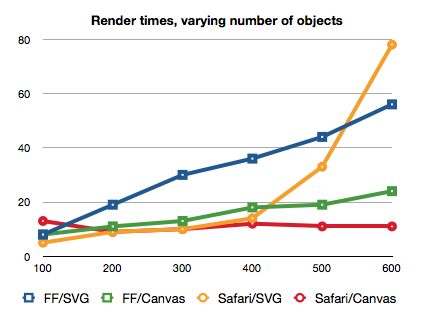
\includegraphics[width=1\textwidth]{Figures/tech-svg-canvas-compare-2.png}
\end{subfigure}%
\begin{subfigure}{.5\textwidth}
  \centering
  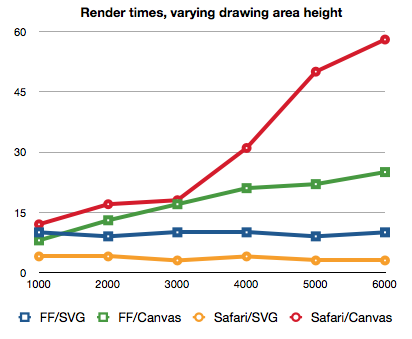
\includegraphics[width=1\textwidth]{Figures/tech-svg-canvas-compare-1.png}
\end{subfigure}
\caption{Performance comparison of Canvas and SVG\cite{CanvasSVGcompare}}
\label{fig:perf-comp-canvas-svg-tech}
\end{figure}

The result of the first experiment, which tested the rendering time of Canvas and SVG with increasing amount of components drawn on it, clearly shows that SVG performance degrades dramatically in the number of objects. However, Canvas performance remains at a near-constant low. The reason is that Canvas is just a bitmap buffer, while SVG has to maintain additional references to each element of object rendered.

On the right of the figure, the second experiment reveals  that canvas performance degrades significantly with varying the size of the drawing area. On the other side, SVG performance is not affected completely. Canvas rendering performance seems to decrease  linearly in the amount of pixels in the canvas area. However, combining two dimensions, Canvas still achieves the better rendering performance.
